\documentclass{article}
\usepackage[a4paper]{geometry}% just for the example
\usepackage[placment=top]{background}
\usepackage{draftwatermark}
\usepackage{tikz}
\usepackage{xcolor}
\backgroundsetup{%
  scale=1,       %% Size - change accordingly
  angle=0,       %% change accordingly
  opacity=0.4,    %% change accordingly
  color =black,  %% change accordingly
  position={7,-7},
  contents={\includegraphics[width=0.5\paperwidth,height=0.35\paperheight]{BirdLogo.png}
    }%}    
    }
    
\definecolor{birdcolor}{RGB}{0,128,128}
\definecolor{eyecolor}{RGB}{55,200,113}
\begin{document}
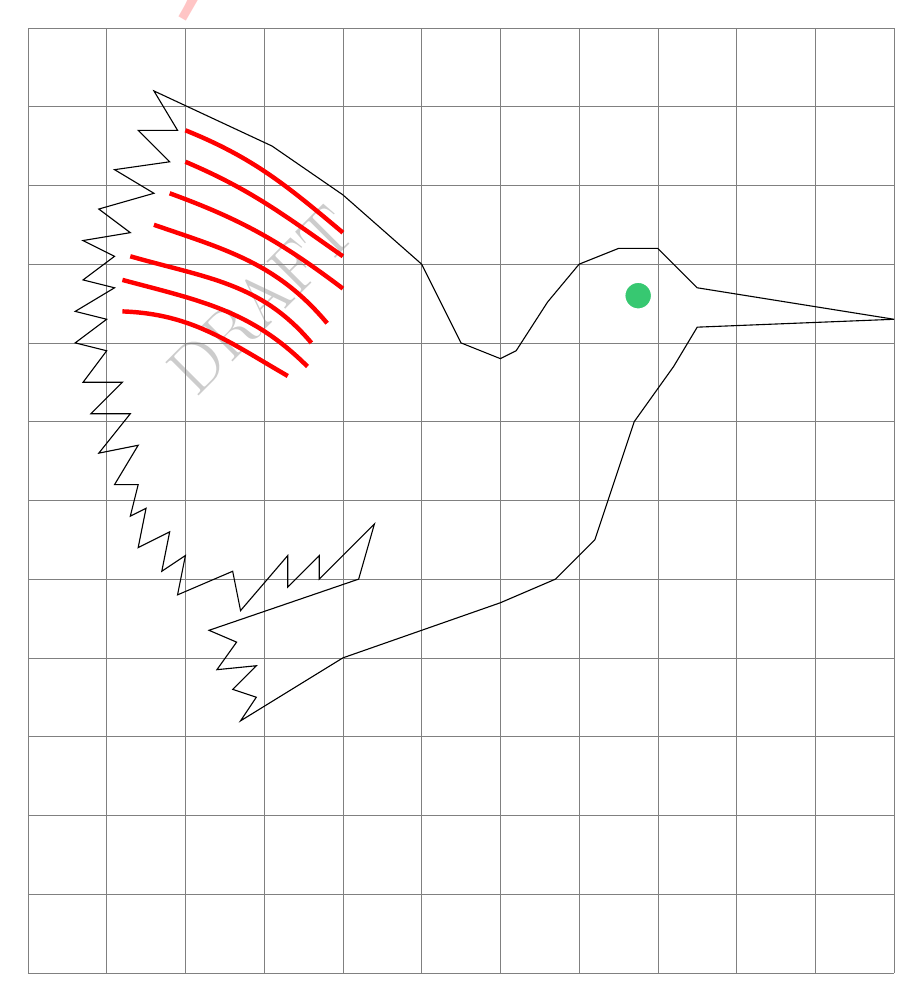
\begin{tikzpicture}
\draw[step=1cm,gray,very thin] (-12,-2) grid (-1,10);
\draw (-1,6.3) -- (-3.5,6.7) -- (-4,7.2) -- (-4.5,7.2) 
-- (-5,7) -- (-5.4,6.52) -- (-5.8,5.9) -- (-6,5.8) 
-- (-6.5,6) -- (-7,7) -- (-8,7.88) -- (-8.9,8.5) 
-- (-10.4,9.2) -- (-10.1,8.7) -- (-10.6,8.7)  -- (-10.2,8.3) 
 -- (-10.9,8.2)  -- (-10.4,7.9) -- (-11.1,7.7) -- (-10.7,7.4)
 -- (-11.3,7.3) -- (-10.9,7.1)  -- (-11.3,6.8)  -- (-10.9,6.7)
-- (-11.4,6.4) -- (-11,6.3) -- (-11.4,6) -- (-11,5.9) -- (-11.3,5.5)
-- (-10.8,5.5) -- (-11.2,5.1) -- (-10.7,5.1) -- (-11.1,4.6)
-- (-10.6,4.7) -- (-10.9,4.2) -- (-10.6,4.2) -- (-10.7,3.8)
-- (-10.5,3.9) -- (-10.6,3.4) --(-10.2,3.6) -- (-10.3,3.1)
-- (-10,3.3) -- (-10.1,2.8) -- (-9.4,3.1) -- (-9.3,2.6)
-- (-8.7,3.3) -- (-8.7,2.9) -- (-8.3,3.3) -- (-8.3,3)
-- (-7.6,3.7) -- (-7.8,3) -- (-9.7,2.35) -- (-9.35,2.2)
 -- (-9.6,1.85) -- (-9.1,1.9)  -- (-9.4,1.6) -- (-9.1,1.5)
-- (-9.3,1.2) -- (-8,2) -- (-6,2.7) -- (-5.3,3) -- (-4.8,3.5)
-- (-4.3,5) -- (-3.8,5.7) -- (-3.5,6.2)
-- (-1,6.3)  
%-- (-11.3,7.3)  %-- (-11.3,7.3)
%-- (-11.3,7.3)
  ;
  %%%% bird eye
  \draw[white , fill=eyecolor, opacity = 1,line width = 2.1pt] (-4.25,6.6) circle (0.199);
 %%%%%% white bands
   \draw [ultra thick,red] (-10,8.7) to[out=-22, in=140] (-8, 7.4);
   \draw [ultra thick,red] (-10,8.3) to[out=-23, in=145] (-8, 7.1);
   \draw [ultra thick,red] (-10.2,7.9) to[out=-20, in=143] (-8, 6.69);
   
   \draw [ultra thick,red] (-10.4,7.5) to[out=-19, in=130] (-8.2, 6.25);
   \draw [ultra thick,red] (-10.7,7.1) to[out=-16, in=130] (-8.4, 6);
   \draw [ultra thick,red] (-10.8 ,6.8) to[out=-15, in=135] (-8.45, 5.7);
   \draw [ultra thick,red] (-10.8,6.4) to[out=-2, in=150] (-8.7,5.58);
  
  
   
\end{tikzpicture}


\begin{tikzpicture}
      
      
    \end{tikzpicture}
\end{document}